83. $y=\left|\cfrac{2-x}{4}\right|=\begin{cases}\cfrac{x-2}{4},\ x\geqslant2\\ \cfrac{2-x}{4},\ x<2.\end{cases}$
$$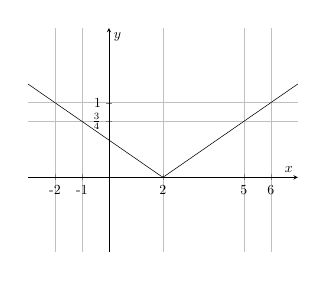
\begin{tikzpicture}[scale=0.5]
\begin{axis}[
    axis lines = middle,
    grid=major,
    legend pos={south west},
    xlabel = {$x$},
    ylabel = {$y$},
    ymin=-1,
    ymax=2,
    xtick={-2,-1,2,5,6},
    xticklabels={-2,-1,2,5,6},
    ytick={0.75, 1},
    yticklabels={$\frac{3}{4}$, 1}            ]
	\addplot[domain=-3:7, samples=100, color=black] {abs((2-x)/4)};
%\addplot[domain=1:6, samples=100, color=black] {x*x-4};
%\addplot[domain=-3.1:2.5, samples=100, color=red] {70*abs(1-2*abs(abs(x)-2))-10*x^2+10*x-70};
	%\addlegendentry{$\text{Рис. 1}$};
\end{axis}
%\draw (3.47,1.89) circle (2pt);
%\draw (3.47,0.63) circle (2pt);
\end{tikzpicture}$$
Исходя из графика, найдём ответ $x\in(-2;6).$\\
